\documentclass[standalone, version=2.0]{huangfusl-template}
\begin{document}
\begin{tabular}{ccc}
    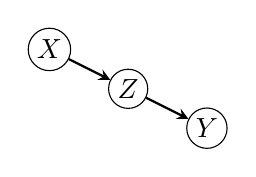
\begin{tikzpicture}
        \node[draw, circle, inner sep=0.5mm] (X) at (0, 0) {$X$};
        \node[draw, circle, inner sep=0.5mm] (Z) at (1, -0.5) {$Z$};
        \node[draw, circle, inner sep=0.5mm] (Y) at (2, -1) {$Y$};
        \draw[thick, -stealth] (X) -- (Z);
        \draw[thick, -stealth] (Z) -- (Y);
    \end{tikzpicture} &
    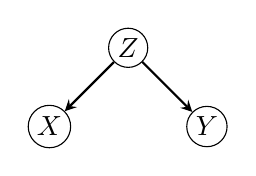
\begin{tikzpicture}
        \node[draw, circle, inner sep=0.5mm] (X) at (0, 0) {$X$};
        \node[draw, circle, inner sep=0.5mm] (Z) at (1, 1) {$Z$};
        \node[draw, circle, inner sep=0.5mm] (Y) at (2, 0) {$Y$};
        \draw[thick, -stealth] (Z) -- (X);
        \draw[thick, -stealth] (Z) -- (Y);
    \end{tikzpicture} &
    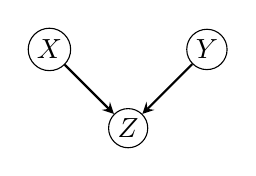
\begin{tikzpicture}
        \node[draw, circle, inner sep=0.5mm] (X) at (0, 0) {$X$};
        \node[draw, circle, inner sep=0.5mm] (Z) at (1, -1) {$Z$};
        \node[draw, circle, inner sep=0.5mm] (Y) at (2, 0) {$Y$};
        \draw[thick, -stealth] (X) -- (Z);
        \draw[thick, -stealth] (Y) -- (Z);
    \end{tikzpicture} \\
    \small \textbf{Chain} & \small \textbf{Fork} & \small \textbf{Collider}
\end{tabular}
\end{document}